\chapter{Processi di supporto}\label{PdS}
\section{Gestione della configurazione}
\subsection{Versionamento}
Per un progetto di tali dimensioni risulta necessario mantenere uno storico completo di tutte le modifiche apportate a qualunque file o documento non generato automaticamente da IDE o simili. Inoltre è necessario uno strumento che permetta il lavoro collaborativo. Per questo scopo si è scelto l'utilizzo del sistema di versionamento \textit{Git$_{G}$}, attraverso il servizio \textit{GitHub$_{G}$}.
\subsubsection{Comandi basilari}
Si riportano di seguito i comandi fondamentali del software Git per fornire un punto di appoggio a tutti i membri del gruppo. Tutti i comandi, tranne quello per la creazione della copia locale, sono da eseguire all'interno della cartella contenente il repository.
\subsubsection{Creazione della copia locale}
La creazione della copia locale viene effettuata attraverso il comando:\\
\texttt{git clone https://github.com/nomeaccount/nomerepostory}.
\subsubsection{Comandi principali}
\begin{itemize}
	\item \texttt{git status}: mostra lo stato del repository locale con i file modificati, i file in area di staging, i file tracciati e non tracciati;
	\item \texttt{git checkout}: permette di cambiare branch attivo nel repository locale;
	\item \texttt{git add nomeFile}: permette di aggiungere un file all'area di staging;
	\item \texttt{git commit -m "Descrizione commit"}: fa il commit dei file presenti in area di staging nel repository locale;
	\item \texttt{git push}: aggiorna sovrascrivendo il repository remoto con quello locale;
	\item \texttt{git pull}: aggiorna sovrascrivendo il repository locale con quello remoto.
\end{itemize}
\subsubsection{Git Flow}
Per facilitare la collaborazione si sceglie usare il git flow\footnote{\url{https://it.atlassian.com/git/tutorials/comparing-workflows/gitflow-workflow}} \textit{workflow$_{G}$}. L'Amministratore si assicurerà che tutte le macchine siano configurate correttamente per il suo utilizzo.
\subsubsection{Gestione dei rilasci}
L'amministratore si occuperà di creare i rami di feature necessari per una proficua collaborazione tra i membri nel repository. Ogni documento (o parte di esso) e ogni funzionalità software verrà implementata in un ramo di feature. Quando la funzionalità diventa stabile e corretta verrà rilasciata in un ramo di integrazione chiamato "develop". Prima di ogni revisione verrà effettuato un rilascio nel ramo master a partire dall'ultimo commit. Tale rilascio costituirà\glossario{baseline}e sarà punto di partenza verso la prossima \textit{milestone$_{G}$}. Tale attività verrà effettuata nei tempi descritti nel \textit{Piano di Progetto v3.0.0}. 

\section{Documentazione}
Il\glossario{processo}di Documentazione stabilisce una serie di norme e convenzioni per la stesura dei documenti così da renderli formali, validi e coerenti.
Un documento viene definito formale quando viene approvato dal \textit{Responsabile}.
Ogni documento formale verrà classificato come:
\begin{itemize}
	\item \textbf{Interno:} documenti ad uso esclusivo del gruppo \textit{ZeroSeven$_{G}$}, quali \textit{Norme di progetto} e \textit{Studio di fattibilità};
	\item \textbf{Esterno:} documenti consultabili anche da attori esterni al gruppo ZeroSeven.
	
\end{itemize}

\subsection{Nomenclatura}
Tutti i documenti formali, esclusi i verbali, seguiranno questo sistema di nomenclatura:
\begin{itemize}
	\item \textbf{Nome del documento:} Il nome del documento deve essere scritto in \textit{Upper Camel Case$_{G}$}.
	NormeDiProgetto per il documento corrente;
	\item \textbf{Versione:} La documentazione prodotta deve essere corredata del numero di versione secondo la seguente codifica:
	
	\textbf{v.X.Y.Z}
	
	dove:
	\begin{itemize}
		\item \textbf{X:} indica il numero crescente di uscite formali. Sarà compito del Responsabile azzerare gli indici Y e Z ad ogni rilascio;
		\item \textbf{Y:} indica lo stato del documento secondo la seguente numerazione:
		\begin{enumerate}
			\setcounter{enumi}{-1}
			\item per la documentazione in fase di sviluppo;
			\item per la documentazione in fase di \textit{verifica$_{G}$};
			\item per la documentazione in fase di approvazione;
			\item per la documentazione approvata e formale.
		\end{enumerate}
		\item \textbf{Z:} indica il numero crescente di modifiche apportate al documento. Ogni modifica deve essere riscontrabile con il diario delle modifiche. Deve essere azzerato quando il responsabile approva il documento. 	
	\end{itemize}
\end{itemize}

I documenti verranno citati secondo il formato NomeDocumento v.X.Y.Z mentre i file saranno rinominati \texttt{NomeDocumento\_v.X.Y.Z.pdf} \\
I verbali sia interni che esterni seguiranno la nomenclatura VerbaleUsoData.

\subsection{Ciclo di vita della documentazione}
Ogni documento formale deve passare gli stadi di ``Sviluppo”, ``Verifica” e ``Approvato”.
\begin{itemize}
	\item \textbf{Sviluppo:} inizia con la creazione del documento e termina con la conclusione	della stesura di tutte le sue parti. In questa fase i Redattori aggiungono le parti assegnate tramite \textit{ticket$_{G}$};
	
	\item  \textbf{Verifica:} il documento entra nella fase di verifica dopo l’assegnazione di un ticket a un \textit{Verificatore} da
	parte del \textit{Responsabile}. I \textit{Verificatori} effettueranno le procedure di controllo
	dello stesso.
	Al termine del controllo in caso positivo il documento entra automaticamente
	in fase di ``Approvazione”, altrimenti i loro riscontri vengono consegnati
	al \textit{Responsabile}, che provvederà ad assegnare nuovamente il
	documento ad un Redattore attraverso una nuova fase di Sviluppo;
	
	\item  \textbf{Approvazione:} l’approvazione di un documento coincide con il superamento
	positivo della verifica.
	Sarà onere del Responsabile decidere, dopo un attenta lettura, se approvare il documento per il rilascio esterno o se è necessario modificare il documento;

	
	\item  \textbf{Approvato:} il documento è pronto per il rilascio esterno.
\end{itemize}


\subsection{Struttura dei documenti}
Al fine di uniformare la struttura grafica e di permettere ai membri del gruppo di concentrarsi solo sulla stesura del contenuto è stato creato un template \LaTeX.
Ogni documento sarà composto da:
\begin{itemize}
	\item Frontespizio;
	\item Diario delle modifiche;
	\item Indice;
	\item Elenco delle immagini e tabelle (se presenti);
	\item Contenuto delle pagine interne.
\end{itemize}
\subsubsection{Frontespizio}
La prima pagina di tutti i documenti dovrà essere così composta:
\begin{itemize}
	\item Titolo del \textit{progetto$_{G}$};
	\item Titolo del documento;
	\item Logo e nome del gruppo;
	\item Descrizione in forma tabellare contenente informazioni importanti quali:
	\begin{itemize}
		\item Versione del documento;
		\item Data di Redazione;
		\item Redattore;
		\item \textit{Verifica$_{G}$};
		\item Approvazione;
		\item Uso;
		\item Distribuzione;
		\item Email di contatto.
	\end{itemize}
\end{itemize}

\subsubsection{Registro delle modifiche}
Successivo al frontespizio deve essere sempre presente un registro riassuntivo delle modifiche del documento in forma tabellare contenente:
\begin{itemize}
\item Versione dopo la modifica;
\item Data della pubblicazione della modifica;
\item Breve descrizione della modifica effettuata;
\item Autore della modifica;
\item Ruolo.
\end{itemize}
\subsubsection{Indice}
Tutti i documenti, eccezion fatta per i verbali, devono contenere un indice il quale permette una visione macroscopica del contenuto del documento,
permettendo una lettura ipertestuale e non necessariamente sequenziale.
 \subsubsection{Elenco delle immagini e tabelle} 
Dopo il diario delle modifiche di ogni documento dovrà essere presente un \textit{Elenco delle figure} ed un \textit{Elenco delle tabelle}.

\subsubsection{Struttura delle pagine interne}
Le pagine interne dei documenti rispettano i canoni previsti dal template \LaTeX e oltre al contenuto interno sono composte da: \\

\begin{itemize}
	\item \textbf{intestazione:}
	\begin{itemize}
		\item logo del gruppo posto a sinistra;
		\item nome del capitolo corrente a destra. 
	\end{itemize}
	\item \textbf {Piè di pagina:}
	\begin{itemize}
	\item titolo del documento completo di versione, posto a sinistra;
	\item numero di pagina posto a destra.
	\end{itemize}

\end{itemize} 
\subsection{Norme tipografiche}
Questa sezione racchiude le convenzioni riguardanti tipografia, ortografia e uno stile uniforme e disciplinato per tutti i documenti.
\subsubsection{Punteggiatura}
Ogni segno della punteggiatura va sempre unito all'ultima lettera della parola che lo precede e separato con uno spazio dalla lettera iniziale della parola che lo segue.
Le lettere maiuscole vanno poste solo dopo il punto, il punto di domanda, il punto esclamativo e all’inizio di ogni elemento di un elenco puntato, oltre che dove previsto dalla lingua italiana. È inoltre utilizzata l’iniziale maiuscola nel nome del team, del \glossario{progetto}, dei documenti, dei ruoli di progetto e delle fasi di lavoro.
\subsubsection{Formati}
\begin{itemize}
\item  Date: le date presenti nei documenti devono seguire la notazione definita dallo standard ISO 8601:2004 YYYY-MM-DD dove:
\begin{itemize}
	\item  YYYY: rappresenta l’anno scritto utilizzando quattro cifre;
	\item MM: rappresenta il mese scritto utilizzando due cifre;
	\item DD: rappresenta il giorno scritto utilizzando due cifre.
\end{itemize}
  \item  Monospace: sarà utilizzato il carattere monospace per formattare il testo contenente parti di codice, comandi, nomi di classi;
  \item  Percorsi: per gli indirizzi email e web  deve essere utilizzato il comando
  \LaTeX \textbackslash url, mentre per gli indirizzi relativi va usato il formato monospace;
  \item Maiuscolo: l'utilizzo del carattere maiuscolo per l'intera parola è riservato esclusivamente agli acronimi.
\end{itemize}
\subsubsection{Stile del testo}
\begin{itemize}
	\item \textbf{Corsivo:}
	il corsivo deve essere utilizzato esclusivamente nei seguenti casi:
	\begin{itemize}
		\item Ruoli: Dovrà essere utilizzato il corsivo quando si parla di ruoli di progetto (es. \textit{Analista});
		\item Documenti: Il nome di un documento andrà scritto in corsivo (es. \textit{Norme di progetto}).
	\end{itemize}
	\item  \textbf{Grassetto:} il grassetto può essere utilizzato esclusivamente negli elenchi puntati per dare risalto al concetto sviluppato;
	\item  \textbf{Sottolineato:} Non è previsto l'uso del testo sottolineato.
	\end{itemize}
\subsubsection{Norme redazionali} 
\label{NormeRedazionali}
\begin{itemize}
	\item \textbf{Elenchi:} Al termine di ogni punto di un elenco verrà utilizzato il carattere (;) eccetto per l'ultimo punto per il quale verrà utilizzato il carattere (.);
	\item \textbf{Riferimenti informativi:} Ogni riferimento a\glossario{prodotti}, guide, software,
	libri esterno al progetto dovrà essere indicato tramite un’annotazione a piè di pagina;
	\item \textbf{\LaTeX:} Ogni riferimento a \LaTeX verrà scritto utilizzando il comando \texttt{\textbackslash LaTeX};
	\item \textbf{Comandi \LaTeX:} sono stati realizzati dei comandi personalizzati al fine di evitare errori di battitura e unificare tutti i documenti facilitando il lavoro del gruppo.
	\begin{itemize}
		\item \textbf{ \textbackslash intestazioni}: inserisce un'intestazione personalizzata con il nome del documento e il logo \textit{ZeroSeven$_{G}$};
		\item \textbf{ \textbackslash mailzeroseven}: inserisce l'indirizzo email del gruppo per un eventuale contatto;
		\item \textbf{ \textbackslash progetto}: inserisce il nome del \textit{progetto$_{G}$};
		\item \textbf{ \textbackslash logo}: inserisce il logo del gruppo ZeroSeven;
		\item \textbf{ \textbackslash glossario}: indica un termine da inserire nel glossario(marcato da una G maiuscola a pedice);
		\item \textbf{\textbackslash analisideirequisiti}: indica il documento \textit{Analisi dei Requisiti} con numero di versione attuale;
		\item \textbf{\textbackslash pianodiqualifica}: indica il documento \textit{Piano di Qualifica} con numero di versione attuale;
		\item \textbf{\textbackslash pianodiprogetto}: indica il documento \textit{Piano di Progetto} con numero di versione attuale;
		\item \textbf{\textbackslash glossariodocumento}: indica il documento \textit{Glossario} con numero di versione attuale;
		\item \textbf{\textbackslash normediprogetto}: indica il documento \textit{Norme di Progetto} con numero di versione attuale;
		\item \textbf{\textbackslash manualesviluppatore}: indica il documento \textit{Manuale dello Sviluppatore} con numero di versione attuale;
		\item \textbf{\textbackslash manualeutente}: indica il documento \textit{Manuale Utente} con numero di versione attuale;
	\end{itemize}
	
	\item \textbf{Sigle:} Nonostante sarà preferito l'utilizzo delle parole per intero potranno essere utilizzate le seguenti sigle:
	\begin{itemize}
	\item ADR = Analisi dei Requisiti;
	\item NDP = Norme di Progetto;
	\item PDP = Piano di Progetto;
	\item PDQ = Piano di Qualifica;
	\item SDF = Studio di Fattibilità;
	\item RR = Revisione dei Requisiti;
	\item RQ = Revisione di Qualifica;
	\item RP = Revisione di Progetto;
	\item RA = Revisione di Accettazione.
	\end{itemize}
\end{itemize}
\subsubsection{Componenti grafiche}
	\begin{itemize}
	\item \textbf{Tabelle:} 
	Ogni tabella presente all'interno dei documenti deve essere accompagnata da una didascalia,	in cui deve comparire un numero identificativo incrementale per la tracciatura della stessa all'interno del documento;
	\item \textbf{Immagini:}
	Le immagini presenti all'interno dei documenti devono essere nel formato Scalable Vector Graphics (\textit{SVG$_{G}$}). In questo modo si garantisce una maggior qualità dell'immagine in caso di ridimensionamento. Per consentire l’inclusione delle immagini nei documenti,
	le immagini dovranno essere convertite nel formato PDF. Qualora non sia possibile
	salvare le immagine in formato vettoriale è preferito il formato Portable Network
	Graphics (PNG).
	\end{itemize}
\subsection{Strumenti a supporto della documentazione}
Per la scrittura della documentazione in modo coerente e uniforme si deve usare il linguaggio di markup \LaTeX.
\subsubsection{TeXstudio}
\`{E} utilizzato per la scrittura e il controllo ortografico dei documenti.
\subsubsection{Script automatici}
Viene implementato uno script per permettere il calcolo automatico dell'\textit{indice di Gulpease$_{G}$}, esso verrà eseguito ad ogni commit tramite \textit{Travis CI$_{G}$}, nel caso in cui la build presenti degli errori grammaticali, essi dovranno essere immediatamente corretti.\\
Aggiungere, se necessario, i termini mancanti nel file \texttt{.dictionary}, contenente i termini che lo script deve ignorare.

\section{Garanzia di qualità}
\subsection{Classificazione metriche e obiettivi}
\label{MetricheObbiettivi}
Questa\glossario{processo}definisce norme e struttura delle metriche, obiettivi di qualità, metodologie e strumenti per perseguire qualità di processo e di prodotto. 
Per mantenere il documento il più ordinato e pulito possibile, la descrizione delle metriche è riportata nell'appendice \S\ref{Metriche}.
\subsubsection{Classificazioni degli obiettivi} 
Gli obiettivi di qualità inclusi nel \pianodiqualifica devono rispettare la seguente notazione: \\
\begin{center}
Q[Tipo][ID] : [Nome].
\end{center}
\begin{itemize}
	\item \textbf{Tipo}: stabilisce se l'obiettivo si riferisce a\glossario{prodotti}o processi e può assumere i seguenti valori:
	\begin{itemize}
		\item \textbf{P}: per indicare i processi;
		\item \textbf{PR}: per indicare i prodotti.
	\end{itemize}
	\item \textbf{ID}: identifica univocamente l'obiettivo attraverso un numero progressivo;
	\item \textbf{Descrizione}: breve descrizione dell'obiettivo di qualità.
\end{itemize}
\subsubsection{Classificazione delle metriche}
Risulta importante fissare delle metriche per permettere di monitorare costantemente la qualità di prodotto e processo. Tali metriche dovranno rispettare la seguente notazione:\\
\textbf{M[Tipo][ID] : [Nome]}
\begin{itemize}
	\item \textbf{Tipo}: stabilisce se la metrica si riferisce a prodotti o processi e può assumere i seguenti valori:
	\begin{itemize}
		\item \textbf{P}: per indicare i processi;
		\item \textbf{PR}: per indicare i prodotti.
	\end{itemize}
	\item \textbf{ID}: identifica univocamente la metrica attraverso un numero progressivo;
	\item \textbf{Descrizione}: breve descrizione della metrica.
\end{itemize}

\subsection{Metriche per la qualità di processo}\label{processo}
Verranno utilizzate le seguenti metriche per valutare l'efficienza e l'efficacia 
processi.

\subsubsection{MP001 - Schedule Variance}
Fornisce una misura di quanto lo stato del progetto è in ritardo o in anticipo rispetto alla pianificazione delle attività.
Essa è il risultato della seguente formula:\\
\begin{center}
	$SV = ${ BCWP} $-${BCWS}
\end{center}
Dove:
\begin{itemize}
	\item \textbf{ BCWP ( Budget Cost of Work Performed )}: è il valore (in giorni o euro) delle attività realizzate alla data corrente. Rappresenta il valore prodotto dal progetto ossia la somma di tutte le parti completate e di tutte le porzioni completate delle parti ancora da terminare;
	\item \textbf{ BCWS ( Budget Cost of Work Scheduled )}: è il costo pianificato (in giorni o Euro) per realizzare le attività di progetto alla data corrente.
\end{itemize}

\subsubsection{MP002 - Cost  Variance }
Indica se si è speso più o meno di quanto è stato previsto.
Il Cost Variance è dato dalla seguente formula:\\
\begin{center}
	$CV = ${ BCWS} $-${ACWP}
\end{center}
Dove:
\begin{itemize}
	\item \textbf{ BCWS ( Budget Cost of Work Scheduled )}: è il costo pianificato (in giorni o Euro) delle attività svolte ad una certa data; 
	\item \textbf{ ACWP ( Actual Cost of Work Performed )}: è il costo effettivamente sostenuto (in giorni o Euro) dalle attività svolte a tale data.
\end{itemize}

\subsubsection{MP003 - SPICE capability level}
Per ogni processo, lo standard 15504 definisce 6 livelli di maturità (da 0 a 5) determinati da un processo di \textit{Process Assessment} che ha lo scopo di determinare l'effettiva qualità dei processi in uso, un processo raggiunge la sua massima efficacia quando raggiunge il livello 5 (raggiunge quindi l'ottimalità).

\subsubsection{MP004 - SPICE process attributes}
Per ogni attributo di processo, lo SPICE definisce 4 livelli (N-P-L-F) di ottimalità riferiti all'attributo stesso, il valore viene dedotto in base ai risultati delle metriche adottate per ciascun processo, un processo raggiunge il livello massimo quando tutte le metriche a lui riferite presentano risultati circoscritti al range di ottimalità definito.

\subsubsection{MP005 - Occorrenza rischi non previsti}
Contatore che viene incrementato all'occorrenza di un rischio non elencato nell'analisi dei rischi del \textit{Piano di Progetto}, un alto valore indica l'eccessiva occorrenza dello stesso e la necessità di un'analisi al fine di mitigare il suo impatto nell'attività di progetto.\\
Viene resettato ad ogni inizio di una nuova fase del progetto.

\subsubsection{MP006 - Indisponibilità dei servizi}
Contatore che viene incrementato ogni qualvolta uno strumento esterno risulta inutilizzabile a causa di errori non gestibili dai membri del gruppo.\\
Viene resettato ad ogni inizio di una nuova fase del progetto.

\subsubsection{MP007 - Complessità ciclomatica}
Metrica software che indica la complessità di un programma tenendo in considerazione moduli, funzioni, metodi e classi.
Nello specifico, essa è calcolata tramite il grafo di controllo di flusso del programma, dove i nodi sono gruppi indivisibili di istruzioni e gli archi connettono due nodi se il secondo gruppo di istruzioni può essere eseguito immediatamente dopo il primo, e il suo valore è determinato dal numero di cammini linearmente indipendenti all'interno del codice sorgente.\\
\'E quindi opportuno definire un valore di complessità ciclomatica preciso: valori alti sono indice di scarsa manutenibilità del codice mentre valori bassi potrebbero indicare scarsa efficienza dei metodi.
Esso fornisce, inoltre, un indice del carico di lavoro richiesto per la fase di testing (un valore alto richiede più test per una copertura completa).\\
Il range di ottimalità stabilito varia da 0 a 10, come suggerito dall'ideatore della metrica Thomas J. McCabe.  

\subsubsection{MP08 - Numero di parametri per metodo}
Definire un range relativo al numero di parametri permette di individuare possibili errori nella progettazione (nel caso in cui un metodo abbia un numero di parametri eccessivo).

\subsubsection{MP009 - Numero di livelli di annidamento}
Metrica per indicare il numero di chiamate annidate di procedure controllate all'interno dei metodi.\newline
Un valore elevato è indice di un basso livello di astrazione del codice e una complessità eccessivamente elevata. 

\subsubsection{MP010 - Attributi per classe}
Un numero elevato di attributi in una classe potrebbe essere indice di un errore di progettazione.
Viene quindi definita una metrica che identifichi range accettabili e ottimali per questo parametro.
Nel caso in cui una classe abbia un numero eccessivo di parametri, valutare la possibilità di suddividere la stessa in più classi, suddividendo quindi le funzioni ad essa assegnate.

\subsubsection{MP011 - Tempo medio del team di sviluppo per la risoluzione di errori}
Indica la quantità di tempo medio utilizzato per risolvere un bug dal team di sviluppo, utile per capire l'impatto medio dell'introduzione di un bug sui tempi di sviluppo. Si misura applicando la seguente formula:
\begin{center}
	\vspace{1em}
	$\frac{\mbox{tempo totale speso per la correzione dei difetti}}{\mbox{numero totale di bug trovati}}$
\end{center}


\subsubsection{MP012 - Efficienza della progettazione dei test}
Indica il tempo medio per la scrittura di un test, un numero troppo elevato potrebbe indicare che si stanno progettando test troppo complessi o che si sta cercando di testare  parti del codice superflue. Si calcola secondo la seguente regola:
\begin{center}
	\vspace{1em}
	$\frac{\mbox{numero totale di test progettati }}{\mbox{tempo per la loro stesura}}$\\
\end{center}


\subsubsection{MP013 - Percentuale build superate}
Ogni build viene controllata tramite script automatici con \textit{Travis CI$_{G}$} e la metrica è il risultato del seguente calcolo:
\begin{center}
	$\frac{\mbox{build superate con esito positivo}}{\mbox{build totali}}$
\end{center}


\subsubsection{MP014 - Media commit giornaliero}
Tale metrica è risultato del seguente calcolo:
\begin{center}
	$\frac{\mbox{commit totali settimanali}}{\mbox{numero giorni settimana}}$
\end{center}


\subsubsection{MP015 - Percentuale requisiti obbligatori soddisfatti}
Tale metrica è risultato del seguente calcolo:
\begin{center}
	$\frac{\mbox{requisiti obbligatori soddisfatti}}{\mbox{requisiti obbligatori totali}}$
\end{center}

\subsubsection{MP016 - Percentuale requisiti desiderabili soddisfatti}
Tale metrica è risultato del seguente calcolo:
\begin{center}
	$\frac{\mbox{requisiti desiderabili soddisfatti}}{\mbox{requisiti desiderabili totali}}$
\end{center}




\subsection{Metriche per la qualità di prodotto}\label{metriche}
Verranno utilizzate le seguenti metriche per valutare l'efficienza e l'efficacia dei
prodotti.
\subsection{MPR001 - Errori ortografici}
Misura il numero di errori ortografici presenti nel documento. La misura viene fatta attraverso script automatici e la verifica da parte dei \textit{Verificatori}.

\subsubsection{MPR002 - Indice di Gulpease}
L’\textit{indice di Gulpease$_{G}$} è un indice di leggibilità di un testo tarato sulla lingua italiana, per il suo calcolo vengono considerate due variabili linguistiche: la lunghezza delle parole e la lunghezza delle frasi rispetto al numero delle lettere.
\begin{center}{$G=89+\frac{300\times N_F-10\times N_L}{N_P}$}\end{center}
$N_F$ indica il numero delle frasi, $N_L$ indica il numero di lettere e $N_P$ indica il numero di parole nel testo.

\subsubsection{MPR003 - Errori inerenti alla correttezza dei documenti}
Misura il numero di errori inerenti alla correttezza del documento. I \textit{Verificatori} hanno il compito di valutare se un documento rispetta le scelte prese dal gruppo.

\subsubsection{MPR004 - Errori inerenti alle Norme di Progetto}
Misura il numero di errori inerenti alle \textit{Norme di Progetto}. I \textit{Verificatori} hanno il compito di valutare se un documento rispetta le \textit{Norme di Progetto}.


\subsubsection{MPR005 - Completezza dell'implementazione funzionale}
Misura la quantità in percentuale di requisiti funzionali soddisfatti dalla corrente implementazione. Viene utilizzata la seguente formula: 
\begin{center}{$CO=\frac{N_{RS}}{N_{RT}}\times 100$}\end{center}
$N_{RS}$  indica il numero di requisiti soddistatti, $N_{RT}$  indica il numero totale di requisiti.

\subsubsection{MPR006 - Correttezza  rispetto alle attese}
Misura la percentuale di risultati affini rispetto alle attese. Viene utilizzata la seguente formula:
\begin{center}{$CRA=(1-\frac{N_{TD}}{N_{TE}})\times 100$}\end{center}
${N_{TD}}$ indica il numero di test che producono risultati discordi rispetto alle attese, ${N_{TE}}$ indica il numero totale di test-case eseguiti.

\subsubsection{MPR007 - Totalità di failure}
Misura la percentuale di test conclusi con una failure. Viene utilizzata la seguente formula:
\begin{center}{$TF=\frac{N_{FR}}{N_{TE}}\times 100$}\end{center}
${N_{FR}}$ indica il numero di failure rilevati durante l'attività di testing,
${N_{TE}}$ indica il numero totale di test-case eseguiti.

\subsubsection{MPR008 - Tempo di risposta}
Misura la differenza media di tempo trascorsa dall’esecuzione di una funzionalità e la restituzione
dell’eventuale risultato. Viene utilizzata la seguente formula:
\begin{center}{$TR=\frac{\sum\limits_{i=1}^n {T_i }}{n}$}\end{center}
${T_i}$ indica il tempo (in secondi) trascorso dalla richiesta di una funzionalità ed il completamento di questa con un eventuale restituzione del risultato.\\

\subsubsection{MPR009 - Comprensibilità  delle funzionalità offerte}
Misura la quantità in percentuale di operazioni comprese dall’utente che non richiedono la
consultazione del manuale. Viene utilizzata la seguente formula:
\begin{center}{$C=\frac{N_{FC}}{N_{FO}}\times 100$}\end{center}
${N_{FC}}$ indica il numero di funzionalità comprese in modo immediato dall'utente, ${N_{FO}}$ indica il numero di funzionalità totali offerte dal sistema.

\subsubsection{MPR010 - Facilità apprendimento}
Misura il tempo medio che occorre ad un utente per imparare ad usare in maniera corretta
una certa funzionalità. Si misura tramite un indicatore numerico che indica i minuti
impiegati da un utente per apprendere il funzionamento di una certa funzionalità;

\subsubsection{MPR011 - Capacità di analisi failure}
Misura la quantità in percentuale di failures incontrate di cui sono state tracciate le cause. Viene
utilizzata la seguente formula:
\begin{center}{$CAF=\frac{N_{FI}}{N_{FR}}\times 100 $}\end{center}
${N_{FI}}$ indica il numero di failure delle quali sono state individuate le cause, ${N_{FR}}$ indica il numero di failures rilevate.

\subsubsection{MPR012 - Impatto delle modifiche}
Misura la quantità in percentuale di modifiche introdotte per risolvere failures che hanno introdotto nuove failures nel prodotto. Viene utilizzata la seguente formula:
\begin{center}{$IM=\frac{N_{FRE}}{N_{FR}}\times 100 $}\end{center}
${N_{FRF}}$ indica il numero di failure risolte introducentro nuove failure, ${N_{FR}}$ indica il numero di failures risolte.





\section{Verifica}
\label{Verifica}
La\glossario{verifica}è un processo atto a evidenziare ed eliminare la possibile presenza di errori.
Di seguito verranno descritti gli strumenti e le pratiche utilizzate per la verifica del codice e dei documenti durante la loro realizzazione.
Durante questa prima fase di progetto la verifica si è focalizzata principalmente su documenti.
\subsection{Verifica di processi}
Ciascun\glossario{processo}verrà costantemente monitorato in tutta la sua esecuzione e documentato alla fine di ogni periodo nell'appendice "Resoconto della verifica" nel \textit{Piano di Qualifica v3.0.0}, secondo le metodologie ISO/IEC 15504.

\subsection{Verifica dei prodotti}
La verifica della qualità di prodotto si divide in attività e procedure differenti a seconda del\glossario{prodotto}che si sta verificando. Per i prodotto software si procede con analisi statica e dinamica, mentre per i documenti si applica soltanto analisi statica.

\subsubsection{Verifica Diagrammi UML}
I \textit{ìVerificatori} devono controllare tutti i diagrammi UML prodotti rispettino lo standard UML e che siano corretti semanticamente.
\subsubsection{Verifica dei documenti}
\paragraph{Analisi statica}
Al fine di verificare i documenti verranno utilizzati\glossario{inspection}e \textit{walkthrough$_{G}$}:
\begin{itemize}
	\item \textbf{Walkthrough:} questa metodologia prevede una lettura profonda e attenta del documento. Gli errori riscontrati verranno corretti e aggiunti all'appendice "Lista di controllo" delle \textit{Norme di Progetto v3.0.0} per permettere di utilizzare inspection le volte successive;
	\item \textbf{Inspection:} al contrario della metodologia precedente, questa risulta essere molto più veloce perché attraverso una lista di controllo degli errori permette un'analisi più efficace delle criticità, omettendo le parti che non presentano problematiche. 
\end{itemize}
Per il controllo dei documenti utilizziamo le funzionalità di TeXStudio assieme a script bash eseguiti da \textit{Travis} per controllare che non ci siano errori nel file \LaTeX\  e verificare l'assenza di errori ortografici. 
\paragraph{Procedura di controllo dei documenti}
\begin{enumerate}
	\item Viene assegnato un\glossario{ticket}a un \textit{Verificatore};
	\item Vengono controllati gli errori comuni attraverso la lista di controllo;
	\item Viene controllato il rispetto delle \textit{Norme di Progetto};
	\item Viene effettuata una lettura profonda e corrette eventuali nuove anomalie;
	\item Calcolo dell'\textit{indice di Gulpease$_{G}$};
	\item Vengono aggiunte eventuali nuove anomalie alla lista di controllo;
	\item Viene chiuso il ticket.
\end{enumerate}
\subsubsection{Verifica del prodotti software}
\paragraph{Analisi dinamica}\label{anDinamica}
\'E compito dei \textit{Progettisti} definire i test nel periodo di progettazione, ad eccezione dei test d'unità(vedi sezione \ref{tunita}); vengono fornite indicazioni specifiche sulla corretta codifica dei test e la loro natura, suddividendo per tecnologie adottate qualora le differenze richiedano un dettaglio maggiore.\\
L'esecuzione dei test automatici tramite \textit{Travis CI$_{G}$} viene avviene unicamente per i test di unità, in quanto il costo computazionale di test di integrazione e di sistema risulta essere troppo elevato.
Per i test riguardanti il back-end (\textit{AWS Lambda$_{G}$} e \textit{API Gateway$_{G}$}), si ricorda che la copertura del codice deve essere totale.
\paragraph{Tecnologie adottate}
\subparagraph{JUnit} Viene adottato per la codifica dei test su \textit{Kotlin$_{G}$}.
\subparagraph{Mocha e Chai Assert} Vengono adottati per la codifica dei test su \textit{Node.Js$_{G}$}: il primo è un\glossario{framework}che fornisce funzioni specifiche e log sul risultato dei test, mentre il secondo ne amplia le funzionalità tramite l'inclusione di una \textit{assertion-library$_{G}$} che rende la sintassi molto più leggibile e facile da codificare.

\paragraph{Test di Unità}\label{tunita}
I test di unità sono del codice prodotto, prodotto dai \textit{Programmatori}, che esercitano un'unità del programma. Per unità si intende una funzionalità atomica che può essere verificata in modo isolato, in modo da assicurare che il risultato del test non sia influenzato da altre unità. 
Vengono sviluppate del programmatore che sviluppa le unità, per verificare l'assenza di alcuni errori, e documentare il comportamento dell'unità prodotta. 
Devono essere veloci da eseguire, indipendenti tra loro e nell'ordine di esecuzione. Inoltre dovrebbero essere eseguiti ad ogni modifica del codice sorgente.
\paragraph{Test di Integrazione}
Il test di integrazione rappresenta l'estensione logica del test di unità. La forma più semplice di questo test prevede la combinazione di due unità già sottoposte a test in un unico componente e il test dell'interfaccia presente fra le due. Il concetto alla base di questo approccio consiste nell'esecuzione di test per la combinazione di più parti, espandendo progressivamente il processo la test di moduli di un gruppo con quelli di altri gruppi. L'obbiettivo finale è di sottoporre al test tutti i moduli che compongono un processo contemporaneamente. 
\paragraph{Test di Sistema}
Il test di sistema sancisce la validazione del prodotto software finale, giunto ad una versione definitiva, e verifica dunque che esso soddisfi in modo completo i requisiti. 
\paragraph{Tracciamento dei test}
Ogni test è strutturato come segue:
\begin{itemize}
	\item Codice identificativo;
	\item Descrizione;
	\item Stato.
\end{itemize}
Il codice identificativo segue la sintassi 
\begin{center}
	\textbf{T\{Tipo\}\{Codice\}}
\end{center}
dove 
\begin{itemize}
	\item \textbf{Tipo}: può essere
		\begin{itemize}
			\item U: se di unità;
			\item I: se di integrazione;
			\item S: se di sistema;
			\item A: se di accettazione.
		\end{itemize}
	\item \textbf{Codice}: può essere
		\begin{itemize}
			\item \textbf{Numerico}: incrementale a partire da 1, associato a test di unità o di integrazione;
			\item \textbf{Di Requisito}: riportando il numero del requisito che testa secondo il tracciamento dei requisiti requisiti presente in \texttt{Analisi dei Requisiti v3.0.0}.
		\end{itemize}
\end{itemize}
	Lo stato di un test può essere:
\begin{itemize}
	\item implementato;
	\item non implementato;
	\item non eseguito;
	\item superato;
	\item non superato.
\end{itemize}
\subsection{Procedure di verifica del software}
\subsubsection{Codifica e esecuzione}
\paragraph{JUnit:}
la struttura di un progetto su \textit{Android-studio$_{G}$} prevede una suddivisione dei test a seconda se richiedano o meno l'ambiente di sviluppo Android per essere eseguiti: i primi sono posizionati nel percorso \textit{app/src/androidTest}, mentre i secondi in \textit{app/src/test}.\\
Alternativamente, è possibile definire un test che utilizzi dei\glossario{Mock}degli oggetti creati dall'ambiente di sviluppo, tuttavia è altamente sconsigliato perché richiederebbe una quantità di lavoro eccessivo e letture successive del codice sarebbero poco intuitive.\\
I test che richiedono l'ambiente di sviluppo\glossario{Android}sono:
\begin{itemize}
	\item test che fanno riferimento a metodi che utilizzano le librerie Android; 
	\item test che richiedono l'utilizzo della rete per essere effettuati; 
	\item test che fanno riferimento a parti dell'interfaccia grafica.
\end{itemize}
I test che non rientrano nelle seguenti categorie (riguardanti, ad esempio, la logica dell'applicazione) possono essere scritti come normali test JUnit nella cartella sopracitata.
\subparagraph{Esecuzione:} L'esecuzione dei test avviene mediante l'invocazione del test con il comando \textit{gradle} [\textit{myTask}] fornito da \textit{gradle$_{G}$}. 

\paragraph{Mocha e Chai Assert:} Mocha permette l'esecuzione seriale di test asincroni mediante l'invocazione di un singolo comando, e rende la loro codifica semplice ed efficace.\\
Segue una lista di direttive da perseguire nella codifica dei test con Mocha:
\begin{itemize}
	\item Evitare l'utilizzo dell'operatore lambda (=>) in tutti i casi, poichè esso non permette al compilatore di Mocha di accedere al contesto delle funzioni a cui fa riferimento, se ciò non risulta necessario, una soluzione che prevede delle lambda porta a difficoltà riguardanti la manutenibilità del codice;
	\item Studiare con cura gli Hooks per la concatenazione dell'esecuzione dei test;
	\item Segnare con la dicitura \textit{Pending} i test non ancora implementati, in modo che i \textit{Progettisti} possano immediatamente identificare i test da codificare;
	\item Evitare di commentare i test da non eseguire, usare invece il comando \textit{skip()}, che da dalla versione 3.0 è supportato anche per i test asincroni;
	\item Evitare l'utilizzo del comando \textit{retries()} del tutto.
\end{itemize}

\subparagraph{Esecuzione:} L'esecuzione avviene mediante l'invocazione del comando \textit{npm test} da terminale. 

\subsubsection{Test per AWS Lambda e Api Gateway}\label{labmdatest}
L'esecuzione dei test sul comportamento delle lambda integrate ad \textit{API Gateway$_{G}$} utilizzate dalla skill e dall'applicazione avviene mediante la console fornita da Amazon\footnote{\url{http://console.aws.amazon.com/}}, che fornisce tutte le informazioni necessarie per verificare il corretto funzionamento delle stesse.
La console, inoltre, viene utilizzata per testare la lambda comunicante con la skill.

\subsubsection{Test sulla skill MegAlexa}
La verifica del corretto funzionamento della skill consiste in un processo comprendente due passi:
\begin{enumerate}
	\item 	\textbf{Test della Lambda:} descritto nella sezione \ref{labmdatest}
	\item \textbf{Test dell'interazione:} tramite la console per sviluppatori fornita da Amazon\footnote{\url{https://developer.amazon.com/alexa/console/ask?}}, è possibile verificare il comportamento della skill prima della sua distribuzione, e simulare un'interazione fra l'utente e Alexa.
\end{enumerate}
\section{Validazione}
\label{Validazione}
Il processo di \glossario{validazione} ha l'obbiettivo di verificare che il prodotto sia conforme a quanto pianificato e sia abile nel gestire e minimizzare gli effetti degli errori.
I passi 

\subsection{Procedura}
Viene descritta la procedura per la validazione delle unità di codice che compongono il prodotto:

\begin{center}
		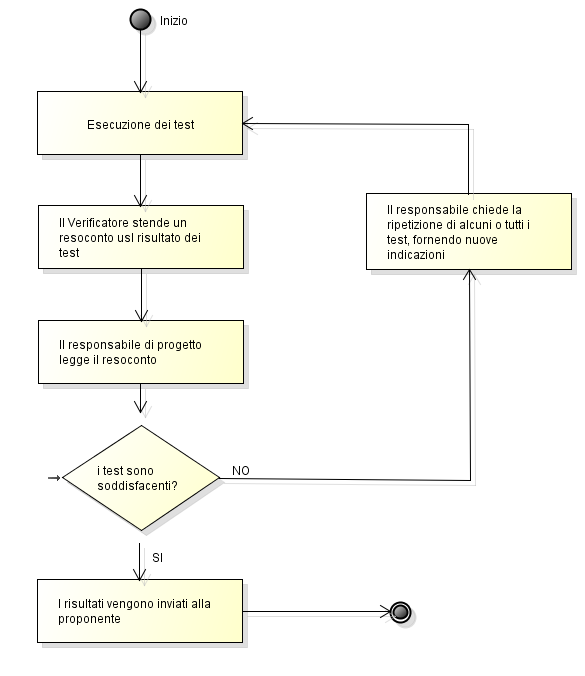
\includegraphics[scale=0.60]{images/uml.png}
\end{center}
